\documentclass[12pt]{article}
 
\usepackage[margin=1in]{geometry} 
\usepackage{amsmath,amsthm,amssymb}
\usepackage{graphicx}
\usepackage{subcaption}
 
\newcommand{\N}{\mathbb{N}}
\newcommand{\Z}{\mathbb{Z}}

\begin{document}

\title{Assignment 2}
\author{Gabriele Stulzer\\ 
Optimisation-Based Robot Control}
 
\maketitle

\section*{Viability Set computation}
 
\subsection*{Question 1}
\textit{}
The states visited with the optimal control trajectory are states that satisfies the system dynamics and constraint, this imposes the feasibility of the states.\\
While starting from a viable state we have an increased likelihood that the visited states are inside the viable kernel, but we are not guaranteed since there are many factors affecting the different states
while executing the trajectory.\\
Evaluating the visited states we can enforce the reliability and feasibility of the computed kernel.\\
If we want to use the visited states to augment the dataset we should first confirm their adheision to the viability constraint but than those states gives valuable new data to the kernel, refining and improving the dataset

\begin{figure}[h!]
    \centering
    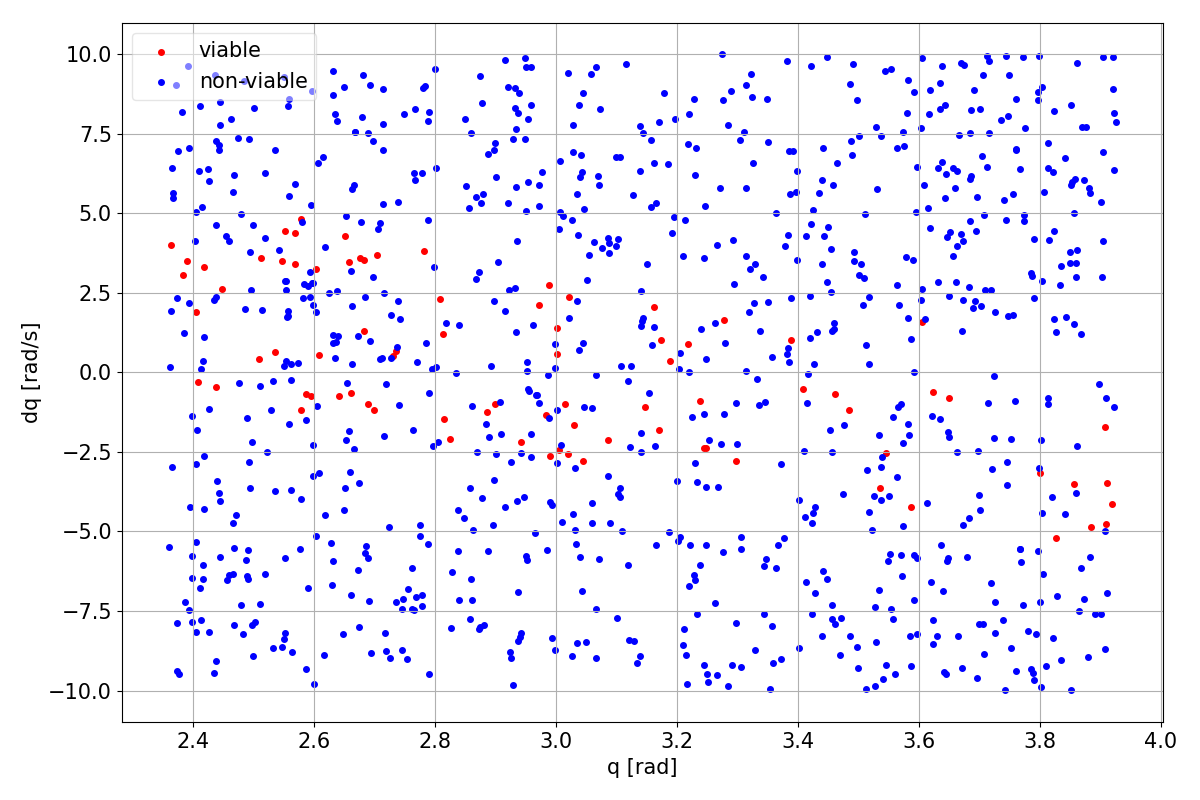
\includegraphics[width=0.5\linewidth]{ViabilityKernelPlot.png}
    \caption{Viability Kernel Plot - 1000 Samples}\label{fig:oscvsic}
\end{figure}

\begin{figure}[h!]
    \centering
    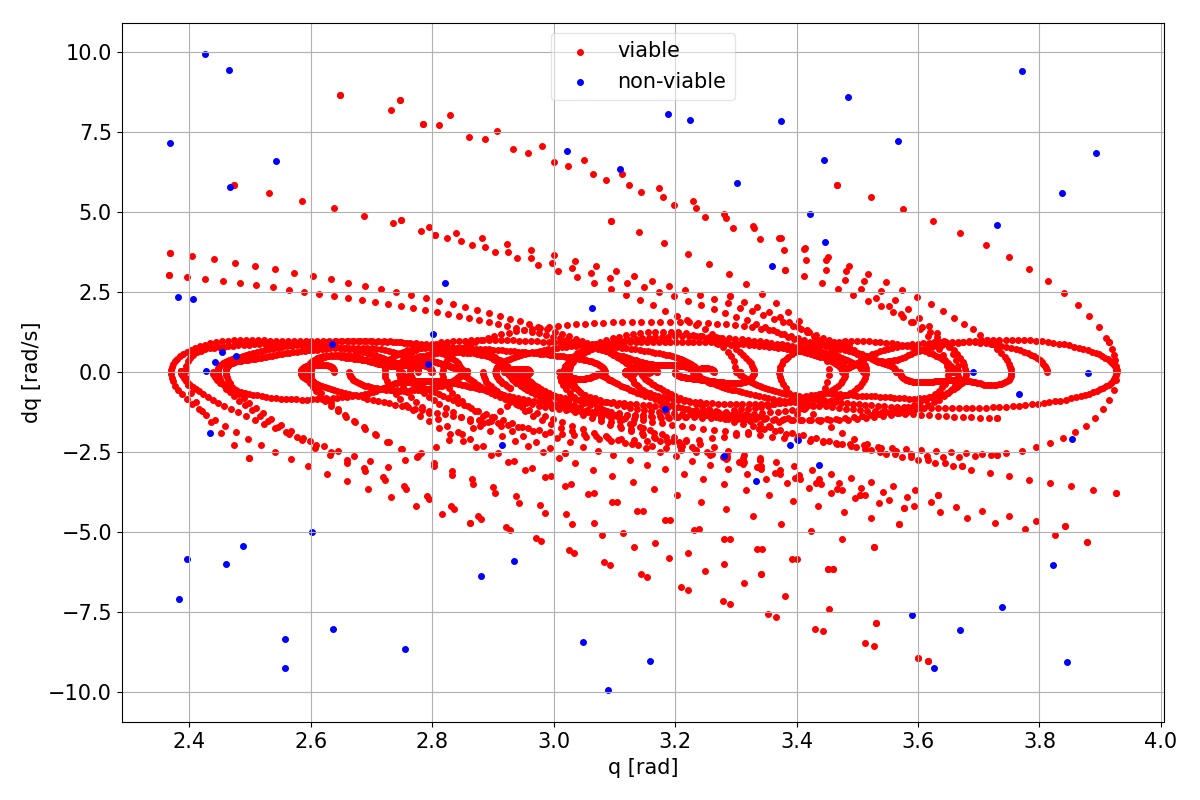
\includegraphics[width=0.5\linewidth]{UsingComputedStatesInKernelSet.png}
    \caption{Viability Kernel Plot with visited states - 1000 Samples | 5g control bounds}\label{fig:oscvsic}
\end{figure}


\subsection*{Question 2}
The shape of the viability kernel is influenced by the control boundaries and the optimal trajectory, we can see that the general shape of the viability kernel follows the one of the optimal trajectory (we can clearly see this in the plot with the visited state added).\\
By increasing or decreasing the control boundaries we can stretch or shrink the width of the region in which we can find the states of the viable set.\\
\begin{figure}[h!]
    \centering
    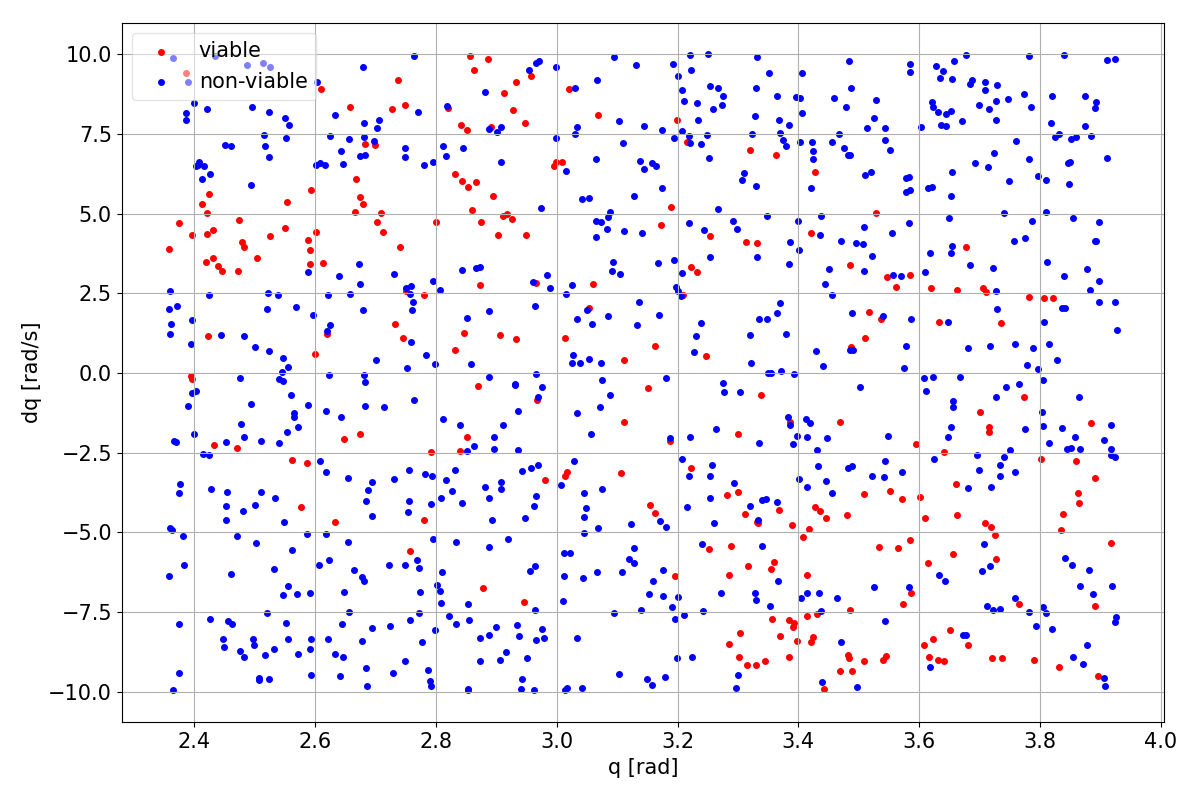
\includegraphics[width=0.5\linewidth]{ViabilityKernelPlot5gcontrolbounds.png}
    \caption{Viability Kernel Plot with increased bounds to 5g - 1000 Samples}\label{fig:oscvsic}
\end{figure}
The bounds of the viability kernel will change depending on the limits we impose, for example how we can see on Figure 4, increasing the velocity bound we get narrower viability kernel boundaries. Reaching in this way a similar effect of increasing the control bounds.


\begin{figure}[h!]
    \centering
    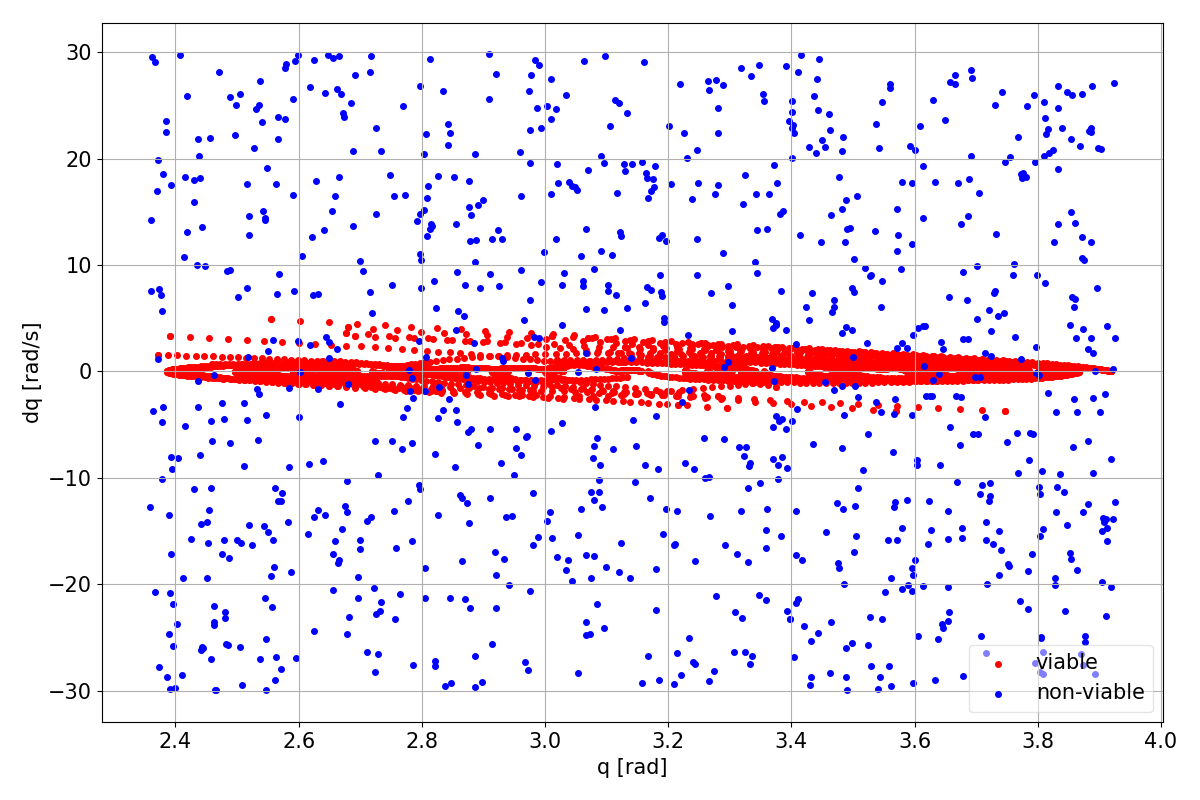
\includegraphics[width=0.5\linewidth]{ViabilityKernelWithIncreasedVelocityBound.png}
    \caption{Viability Kernel Plot with increased Velocity - 1000 Samples}\label{fig:oscvsic}
\end{figure}

\subsection*{Question 3}
The viability kernel is a relevant information, which is very useful in solving the recursive feasibility problem in MPC. One of the easiest way we can exploit this data is to choose a initial state that is inside the viability kernel.\\
Another possible way is to use the control invariant property of the computed set to exploit the theorem about recursive feasibility of MPC that states that if a terminal constraint set is control invariant the MPC problem is recursive feasibile.\\
We could also try to extract information from the boundaries of the viability kernel to incorporate in the MPC problem, this would ensure that the computed trajectories remain within the viable state space, enhancing the recursive feasibility of the controller.\\
With the same information we could optimize the constraints of the problem by refining or tightening them.

\end{document}